\subsection{系统性能测试}
\label{subsec:featurespy-evaluation-performance}

\subsubsection{测试环境}
\label{subsubsec:featurespy-platform}

本文为\prototype 的性能评估配置了以下两个测试平台:

\begin{itemize}[leftmargin=*]
    \item {\bf 本地集群(LAN)。}包括三台设备,每台设备均配备一个八核2.9\,GHz的Intel Core i7-10700 CPU,一个4\,TB 7200转的希捷银河系列SATA机械硬盘32\,GB DDR4内存。所有机器都通过10\,Gbps交换机进行连接,并运行Ubuntu 20.04.3 LTS。
    \item {\bf 云环境(Cloud)。}本文在两个不同区域的阿里云\cite{Alibaba}部署了多台规格为{\tt ecs.g7t.3xlarge}的虚拟机(VM)来分别运行云服务端、密钥服务器和多个客户端。同一地域和不同地域的虚拟机分别通过10\,Gbps和100\,Mbps网络连接。每个虚拟机均配备一个12核3.5GHz的虚拟CPU(底层物理机CPU为Intel Xeon (Ice Lake) Platinum 8369B)和48GiB内存,并安装阿里云Linux 3.2104操作系统。本文另外挂载了阿里云通用存储{\tt Alibaba General-Purpose NAS}作为云服务端的存储后端。该NAS可实现高达15K\,IOPS的4\,K随机读写,且顺序读写性能为150\,MiB/s。
\end{itemize}

本文进行以下默认配置:对于底层\sysnameF,本文固定检测窗口大小$W$=5\,K(需消耗大约300\,KiB安全区内存),报告攻击的阈值$T$=3\%,相似性指标的大小为2个加密块(即,32字节),通过N-transform提取的特征数量为3个。对于\prototype,本文配置了三个线程来提取明文数据块的内容特征(除了 Exp\#5,它使用单个线程对\prototype 中各个模块的性能进行基准测试,而 Exp\#6评估了\prototype 使用不同线程数进行特征提取时的性能),并在云服务端使用了一个大小为1\,GiB容器(云服务端的基本存储单位,参见\S\ref{sec:featurespy-implementation})缓存以提高下载性能。

\subsubsection{合成工作负载}
\label{subsubsec:featurespy-syn}
本文使用SYNUnique评估\prototype 在合成数据集作为工作负载情况下的性能。数据集中每个2\,GiB的随机文件均只包括全局非重复的数据块(\S\ref{subsec:featurespy-datasets})。为了测试\prototype 的峰值性能,本文在每次测试之前将所有数据加载到每个客户端的内存中(避免磁盘I/O的影响),并将云服务端接收到的所有数据存储在内存中(不包含Exp\#8,其包含磁盘I/O以研究真实云环境部署下的系统性能)。实验结果表明\prototype 与本文提出的高性能加密后重复数据删除系统\sysnameS (\S\ref{sec:sgxdedup-implementation})相比仅产生有限的性能开销。本文将每个实验的10次测试的平均结果及其T分布{\tt Student's t-Distribution}95\%置信区间包含在条形图中(为简洁起见,折线图中不包含置信区间)。

\paragraph*{Exp\#5(微基准性能测试)。}
本文通过微基准测试了解\prototype 中各个步骤的计算开销。本实验在LAN测试平台的不同机器上分别部署客户端、密钥服务器和云服务端。本文使用客户端连续上传两次SYNUnique中的同一个2\,GiB随机文件,并在单个线程中评估不同步骤的处理时间。本文考虑的步骤包括:(1)数据分块({\tt chunking}),将输入文件划分为可变大小的明文数据块;(2)特征提取({\tt feature generation}),提取每个明文数据块的内容特征,并根据\sysnameF 的各个实例对目标特征进行采样;(3)数据块指纹计算({\tt fingerprinting}),计算每个明文数据块的指纹;(4)密钥生成({\tt key generation}),生成特征密钥和消息锁加密密钥;(5)加密({\tt encryption}),对每个明文数据块进行保留相似性加密;(6)攻击检测({\tt detection}),基于密文数据块的相似性指标检测推测内容攻击;(7)数据所有权证明({\tt PoW}),证明每个密文数据块的所有权;(8)重复数据删除({\tt deduplication}),云服务端检测数据块是否已被存储,并将结果返回给客户端;(9)数据传输({\tt transfer}),传输不重复的密文数据块和文件元数据。

\begin{table}[!htb]
    \small
    \centering
    \setlength{\tabcolsep}{5pt}
    \renewcommand{\arraystretch}{1.05}
    \setlength{\tabcolsep}{0.006\textwidth}{
        \begin{tabular}{|c|c|c|c|c|}
            \hline
            \multicolumn{2}{|@{\,}c|}{\textbf{步骤/操作}}      & \multicolumn{1}{l|}{\hspace{.5em}\textbf{firstFeature实例}} &
            \multicolumn{1}{c|}{\textbf{minFeature实例}}       &
            \multicolumn{1}{c|}{\textbf{allFeature实例}}                                                                                                    \\ \hline \hline
            \multicolumn{2}{|c|}{数据分块}                     & \multicolumn{3}{c|}{$2.12\pm0.006$}                                                        \\ \hline
            \multicolumn{2}{|c|}{\makecell[c]{特征提取}}       &
            \makecell[c]{$4.34 \pm 0.01$}                      & \makecell[c]{$9.93 \pm0.04$}                                & \makecell[c]{$9.85 \pm0.02$} \\ \hline
            \multicolumn{2}{|c|}{\makecell[c]{数据块指纹计算}} &
            \multicolumn{3}{c|}{$1.81 \pm 0.002$}                                                                                                           \\ \hline        \multicolumn{2}{|c|}{\makecell[c]{密钥生成}}&
            \multicolumn{3}{c|}{$0.73 \pm 0.02$ ($0.49 \pm 0.01$)}                                                                                          \\ \hline
            \multicolumn{2}{|c|}{加密}                         & \multicolumn{3}{c|}{$1.22 \pm 0.001$}                                                      \\ \hline
            \multirow{2}{*}{安全区内}
                                                               & 攻击检测                                                    &
            \multicolumn{3}{c|}{$0.04   \pm 0.005$}                                                                                                         \\ \cline{2-5}
                                                               & 所有权证明                                                  &
            \multicolumn{3}{c|}{$1.86   \pm 0.004$}                                                                                                         \\ \hline
            \multicolumn{2}{|c|}{重复数据删除}                 &
            \multicolumn{3}{c|}{$0.55 \pm 0.02$}                                                                                                            \\ \hline
            \multicolumn{2}{|c|}{数据传输}                     & \multicolumn{3}{c|}{$1.16 \pm 0.03$ ($0.04 \pm 0.001$)}                                    \\ \hline
        \end{tabular}
    }
    \caption{(Exp\#5)每处理1\,MiB数据时各步骤的时间开销(单位:ms)。除括号中明确指出外,第二轮上传的每一步骤所消耗的时间与第一轮上传的相同。}
    \label{tab:featurespy-evaluation-syn-system-breakdown}
\end{table}

表~\ref{tab:featurespy-evaluation-syn-system-breakdown}展示每1\,MiB文件数据处理时各个步骤的时间开销。由于\prototype 建立在\sysnameS(\S\ref{sec:sgxdedup-implementation})之上,它继承了在非首次上传时通过推测性加密降低密钥生成开销(\S\ref{sec:featurespy-implementation})以及避免传输重复数据块带来的性能优势。结果表明,针对推测内容攻击的检测步骤是高效的,并且在上传过程中仅占用了总时间开销的0.4\%。由于N-transform的计算开销,特征生成步骤开销很高。例如,{\tt firstFeature}实例中在第一轮上传时占用了总时间开销的31.4\%;{\tt minFeature}和{\tt allFeature}实例中特征提取所消耗的时间占比分别进一步增加到51.1\%和50.9\%,这是因为它们都提取了所有三个特征(与只需要提取第一个特征的{\tt firstFeature}相反)。然而,本文认为可以通过多线程来减轻特征生成的性能开销对\prototype 整体性能的影响(见下文)。

\paragraph*{Exp\#6(单客户端上传/下载性能)。}
本文考虑单个客户端,并将\prototype 的性能与其基础\sysnameS 进行比较。本文令客户端连续两次上传相同的SYNUnique文件(如Exp\#5),最后下载该文件。

\begin{figure}[!htb]
    \centering
    
\includegraphics[width=0.7\textwidth]{pic/featurespy/plot/performance/LANSyn/legend.pdf}\\
    \vspace{1pt}
    \begin{tabular}{@{\ }c@{\ }c@{\ }c}
        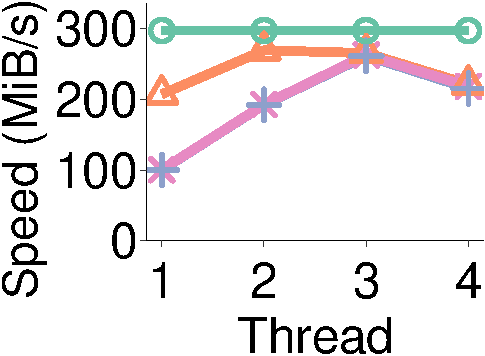
\includegraphics[width=0.3\textwidth]{pic/featurespy/plot/performance/LANSyn/upload_thread_line.pdf}     &
        \hspace{8pt}
        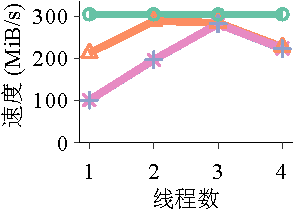
\includegraphics[width=0.3\textwidth]{pic/featurespy/plot/performance/LANSyn/upload_thread_2nd_line.pdf} &
        \hspace{8pt}
        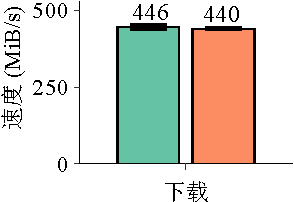
\includegraphics[width=0.3\textwidth]{pic/featurespy/plot/performance/LANSyn/download_bar.pdf}             \\
        \makecell[c]{\small (a)第一轮上传}                                                                       &
        \makecell[c]{\small (b)第二轮上传}                                                                       &
        \makecell[c]{\small (c)下载}                                                                               \\
    \end{tabular}
    \caption{(Exp\#6)LAN测试平台中的单客户端上传/下载性能。在下载中,所有\prototype 的三种实例都达到相同的速度,本文将它们(橙色)与 \sysnameS(绿色)进行比较。}
    \label{fig:featurespy-singleClientThroughput}
\end{figure}

图~\ref{fig:featurespy-singleClientThroughput}(a)和图~\ref{fig:featurespy-singleClientThroughput}(b)分别展示了改变提取特征的线程数(\S\ref{sec:featurespy-implementation})时\prototype 三种实例的性能变化。由于\sysnameS 无需进行特征提取,其第一轮上传速度为297.1\,MiB/s,并在第二轮上传中保持为304.3\,MiB/s。第二轮中上传性能稍有提升,这是由于\sysnameS 可在第二轮中通过推测行加密提升密钥生成速度,且无需上传任何数据块(\S\ref{sec:sgxdedup-implementation})。
\prototype 的上传速度首先随着线程数的增加而增加。随后,{\tt firstFeature}实例在2个线程时达到峰值为265.3\,MiB/s,而{\tt minFeature}和{\tt allFeature}实例在3个线程时达到峰值分别为261.3\,MiB/s和262.6\,MiB/s(第一轮上传),随后由于多线程资源竞争,性能在逐渐下降。在4个线程时,由于多线程资源竞争,对于所有三个实例第一轮上传速度降低至大约为220\,MiB/s,而第二轮上传速度降低至约为225\,MiB/s。

通过利用多线程,\prototype 仅在第一轮上传时相较于\sysnameS 仅产生8.0-12.0\%的额外性能开销,而在第二轮上传时缩减为6.6-7.5\%。此外,本文观察到第一轮(传输所有数据块)和第二轮(不需要传输重复数据)上传之间的性能差异很小,这是因为本文的LAN测试平台具有高带宽来传输数据。本文认为源端重复数据删除在实际云部署中带来了显着的性能提升(Exp\#8),并减少了处理实际存储工作负载的网络流量开销(Exp\#10)。图~\ref{fig:featurespy-singleClientThroughput}(c)比较下载速度。相较于\sysnameS,\prototype 会导致1.3\%的性能下降,这是因为它同时使用消息锁加密密钥和特征密钥解密每个密文数据块。

\paragraph*{Exp\#7(多客户端上传/下载性能)。}
本文评估多个客户端同时发出上传/下载请求时的总体性能。本文使用Cloud测试平台以便测试更多客户端。本文将所有客户端、密钥服务器和云服务端部署在同一个区域。本文将总上传(下载)数据大小与所有客户端完成上传(下载)的总时间的比率记为聚合的上传(下载)速度。

\begin{figure}[!htb]
    \centering
    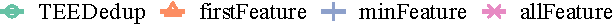
\includegraphics[width=0.7\linewidth]{pic/featurespy/plot/performance/multiClient/legend.pdf}\\
    \vspace{1pt}
    \begin{tabular}{@{\ }c@{\ }c@{\ }c}
        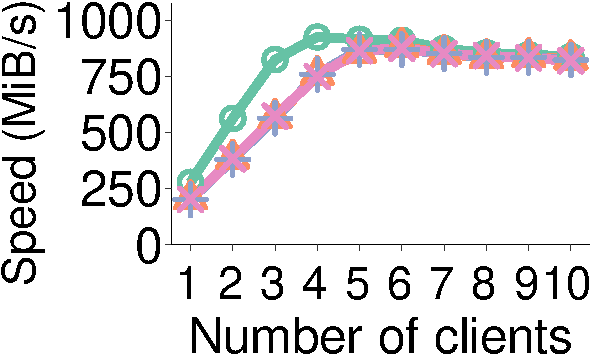
\includegraphics[width=0.32\textwidth]{pic/featurespy/plot/performance/multiClient/upload_1st_line.pdf} &
        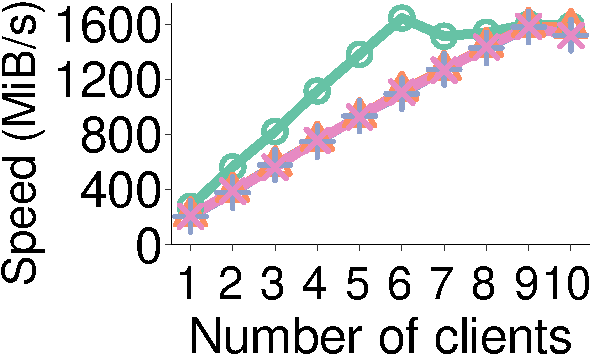
\includegraphics[width=0.32\textwidth]{pic/featurespy/plot/performance/multiClient/upload_2nd_line.pdf} &
        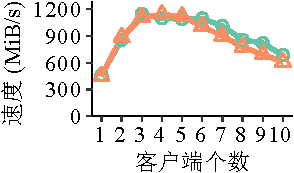
\includegraphics[width=0.32\textwidth]{pic/featurespy/plot/performance/multiClient/download_line.pdf}     \\
        \makecell[c]{\small (a)第一轮上传}                                                                      &
        \makecell[c]{\small (b)第二轮上传}                                                                      &
        \makecell[c]{\small (c)下载}                                                                              \\
    \end{tabular}
    \captionof{figure}{(Exp\#8)多客户端上传/下载性能。所有\prototype 实例的下载速度均相同的,本文将它们(橙色)与 \sysnameS(绿色)进行比较。}
    \label{fig:featurespy-expMultiClientThroughput}
\end{figure}

图~\ref{fig:featurespy-expMultiClientThroughput}给出了至多10个客户端的聚合上传(下载)性能测试结果。本文不考虑更多的客户端,这是因为聚合上传速度已经基本稳定。具体来说,第一轮和第二轮上传的聚合速度都随着客户端数量的增加而增加,随后由于云服务端的写入竞争而逐渐降低。本文观察到\sysnameS (例如,4个客户端的聚合上传速度在第一轮达到924.9\,MiB/s)比\prototype 更早达到峰值性能(例如,6个客户端的聚合上传速度在第一轮中达到882.2\,MiB/s),这是因为\sysnameS 具有更高性能并且云服务端很容易饱和。类似地,由于云服务端的读竞争,\prototype 的三种实例的聚合下载速度均在4个客户端时达到峰值1141.3\,MiB/s,而\sysnameS 则在3个客户端时达到峰值1148.7 MiB/s。

\paragraph*{Exp\#8(云环境上传/下载性能)。}
本文扩展Exp\#6来研究真实云环境(经由互联网进行数据外包)下单客户端的上传/下载性能。本文将客户端和密钥服务器部署在同一地域的两台虚拟机(具体配置参见\S\ref{subsubsec:featurespy-platform})中,并在不同地域的虚拟机部署云服务端(与Exp\#7不同,其所有实体均部署在同一地域,通过局域网连接),从而模拟客户端与云服务端经由互联网连接的场景。此外,本文要求客户端从本地磁盘(即,读写速度约为270\,MiB/s的固态硬盘)读取文件并进行上传,云服务端则将接收到的数据存储在附加的NAS中。本文使用最基本的数据传输工具{\tt scp}将2\,GiB文件从客户端上传到云服务端,作为客户端与云服务端之间的互联网数据传输速度的基准。

\begin{table}[!htb]
    \centering
    \small
    \begin{tabular}{cccc}
        \toprule
        {\bf 方案}                     & {\bf 第一轮上传(非重复数据)}        & {\bf 第二轮上传(重复数据)} & {\bf 下载}                        \\
        \midrule
        网络带宽                       & \multicolumn{3}{c}{11.8 $\pm$ 0.04}                                                                  \\
        \hline
        \makecell[c]{\tt firstFeature} & \multirow{3}{*}{11.5 $\pm$ 0.006}   & 204.4 $\pm$ 10.06          & \multirow{3}{*}{11.5 $\pm$ 0.004} \\
        \makecell[c]{\tt minFeature}   &                                     & 184.7$\pm$ 7.4             &                                   \\
        \makecell[c]{\tt allFeature}   &                                     & 185.0$\pm$ 6.4             &                                   \\
        \hline
        \sysnameS                      & 11.5 $\pm$ 0.009                    & 233.2 $\pm$ 8.4            & 11.5 $\pm$ 0.004                  \\
        \bottomrule
    \end{tabular}
    \captionof{table}{(Exp\#7) 云环境下部署\prototype 的上传/下载性能(单位:MiB/s)}
    \label{tab:featurespy-expCloudTest}
\end{table}

表~\ref{tab:featurespy-expCloudTest}列出了实验结果。在第一轮上传中,所有方法的性能都受到网络带宽的限制(均低于11.9\,MiB/s)。在第二轮上传中,\sysnameS 和{\tt firstFeature}实例的性能受到数据分块(Table~\ref{tab:featurespy-evaluation-syn-system-breakdown})的限制,而{\tt firstFeature}实例相较于\sysnameS 产生了12.3\%的额外性能开销,这是因为它额外提取了每个数据块的第一个特征来生成特征密钥。{\tt minFeature}实例和{\tt allFeature}实例(在第二轮上传中)的性能受特征提取的限制。这里,所有方法的第二轮上传速度都比LAN测试平台中的(Exp\#6)结果慢。原因有三个:首先,本实验包含了磁盘I/O开销;此外,云测试平台中的虚拟机是从物理机虚拟化得到的,在处理计算密集型操作时由于资源隔离等要求可能会导致性能下降;最后,互联网的高延迟减慢了重复数据删除中数据块指纹的传输速度。在下载中,所有方法的性能都受到网络带宽的限制,与\sysnameS 相比,\prototype 会产生约0.6\%的额外性能开销。

\subsubsection{实际工作负载}
\label{subsubsec:featurespy-real}
本文使用4个数据集(参见\S\ref{subsec:featurespy-datasets})评估 \prototype,以了解其在处理真实世界大规模数据时的表现。

\paragraph*{Exp\#9(实际工作负载下的上传/下载性能)。}本文在LAN测试平台上测试真实工作负载下的上传/下载性能,并考虑磁盘I/O的影响。即,客户端从磁盘读取数据集,且云服务端将接收到的所有数据写入磁盘。本文从FSL和MS数据集中分别选取了10个快照。对于FSL,本文选择来自同一用户的每周快照以获得较高的快照间冗余;对于MS,本文选择具有最多快照内冗余的快照。选择的FSL和MS快照逻辑大小分别为407.5\,GiB和902.5\,GiB。由于两个数据集的快照只包含数据块指纹和大小(\S\ref{subsec:featurespy-datasets},本文通过重复将其指纹写入当前数据块指定大小的缓存来重建每个明文数据块。此外,本文不采用Linux和CouchDB数据集,这是因为两者的总数据量较小且具有完整数据内容,其性能表现于合成工作负载性能测试中单客户端的上传下载性能(Exp\#6)表现类似。本文先逐个上传快照,然后按照上传的顺序依次下载所有快照。这里,由于基本的\sysnameS 没有容器缓存(\S\ref{sec:featurespy-implementation});为了公平比较,本文为\sysnameS 增加了与\prototype 相同的大小为1\,GiB的容器缓存。

\begin{figure}[!htb]
    \centering
    
\includegraphics[height=0.2in]{pic/featurespy/plot/performance/LANTrace/trace_legend_upload.pdf}\\
    
\includegraphics[height=0.2in]{pic/featurespy/plot/performance/LANTrace/trace_legend_download.pdf}\\
    \vspace{3pt}
    \begin{tabular}{@{\ }c@{\ }c}
        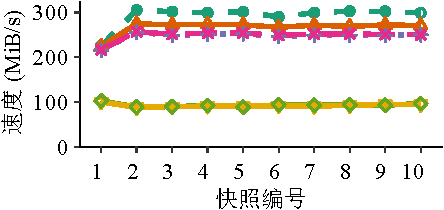
\includegraphics[width=0.47\textwidth]{pic/featurespy/plot/performance/LANTrace/trace_fsl.pdf} &
        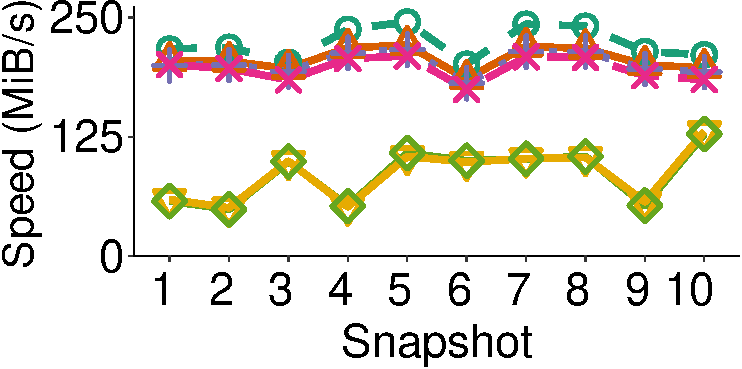
\includegraphics[width=0.47\textwidth]{pic/featurespy/plot/performance/LANTrace/trace_ms.pdf}    \\
        \mbox{\small (a) FSL}                                                                          &
        \mbox{\small (b) MS}                                                                             \\
    \end{tabular}
    \caption{(Exp\#9)实际工作负载下上传/下载性能}
    \label{fig:featurespy-traceDrivenThroughput}
\end{figure}

图~\ref{fig:featurespy-traceDrivenThroughput}展示基于数据集的实际工作负载下\prototype 的性能测试结果。对于FSL数据集,在第一个快照(例如,\sysnameS、{\tt firstFeature}、{\tt minFeature} 和{\tt allFeature}实例分别为224.8\,MiB/s,223.9\,MiB/s,214.9\,MiB/s和216.9\,MiB/s)之后,\sysnameS 和\prototype 都实现了较高的性能(例如,\sysnameS、{\tt firstFeature}、{\tt minFeature}和{\tt allFeature}实例分别不低于298.9\,MiB/s,266.8\,MiB/s,246.4\,MiB/s和248.8\,MiB/s)。这是因为FSL数据集中每个快照之间的冗余度较高,之后的快照上传时很大比例数据块无需上传。两者在FSL数据集中的下载速度基本稳定(例如\sysnameS 为88.7-102.6\,MiB/s,\prototype 为88.0-100.2\,MiB/s)。平均而言,与\sysnameS 相比,{\tt firstFeature}、{\tt minFeature}和{\tt allFeature}实例的上传性能分别降低8.8\%、15.7\%和15.0\%,下载性能降低了0.8 \%。

与FSL数据集相比,MS数据集中的上传性能通常下降约21\%,这是因为MS数据集包含大量非重复的数据块并使得云服务端产生较大的指纹索引(通过LevelDB\cite{leveldb}实现)。这加重了通过指纹索引查询密文数据块是否存在以进行重复数据删除的开销。此外,MS数据集中的下载速度会随着快照的变化而波动,这是因为一些快照具有更多的非重复数据块,并且可能存储在可以通过顺序读取快速访问的连续区域(即数据块碎片较少\cite{lillibridge13})中。

\paragraph*{Exp\#10(网络流量开销分析)。}
本文分析了\prototype 的网络流量开销,并将其与三种可以抵御推测内容攻击的重复数据删除方法进行比较:(1)目标端重复数据删除({\tt target-based deduplication})\cite{harnik2010side},强制客户端传输所有密文数据块到云服务端;(2)随机阈值重复数据删除({\tt random-threshold deduplication})\cite{harnik2010side},如果每个数据块的上传次数小于预定义的阈值,则执行目标端重复数据删除,否则执行源端重复数据删除(\S\ref{sec:background-enc-deduplication});(3)两阶段重复数据删除({\tt Two-stage deduplication})\cite{li15},对来自同一客户端的密文数据块执行源端重复数据删除,然后对跨不同客户端的密文数据块执行目标端重复数据删除。这里,本文按照之前的工作\cite{harnik2010side}分别选择20和2作为随机阈值重复数据删除中阈值的上限和下限。对于FSL数据集,本文根据日期合并每个用户的快照,并按时间顺序存储;对于MS数据集,本文假设每个快照都来自于一个独立的客户端,并按照快照编号的顺序存储;对于Linux和CouchDB数据集,本文假设每个快照来自一个独立的客户端,并按照版本号进行存储。特别的,CouchDB中一次按照通用、企业和社区三个发行版的顺序依次存储。此外,本文不考虑文件元数据导致的带宽开销。

\begin{figure}[!htb]
    \centering
    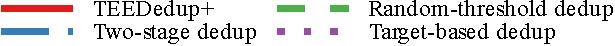
\includegraphics[width=0.65\textwidth]{pic/featurespy/plot/bandwidth/upload_traffic_legend.pdf}     \vspace{3pt} \\
    \begin{tabular}{@{\ }c@{\ }c}
        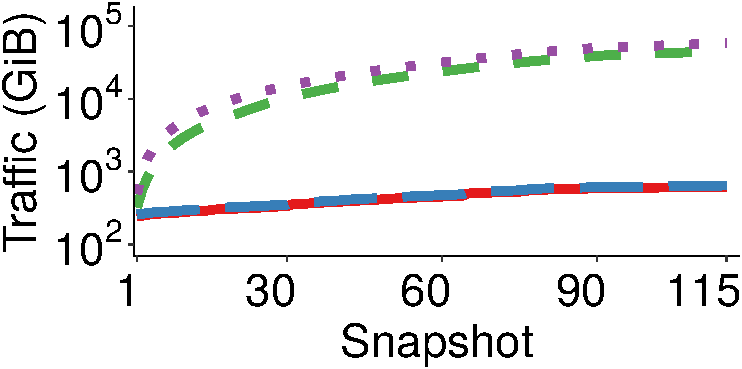
\includegraphics[width=0.47\textwidth]{pic/featurespy/plot/bandwidth/upload_traffic_fsl.pdf}   &
        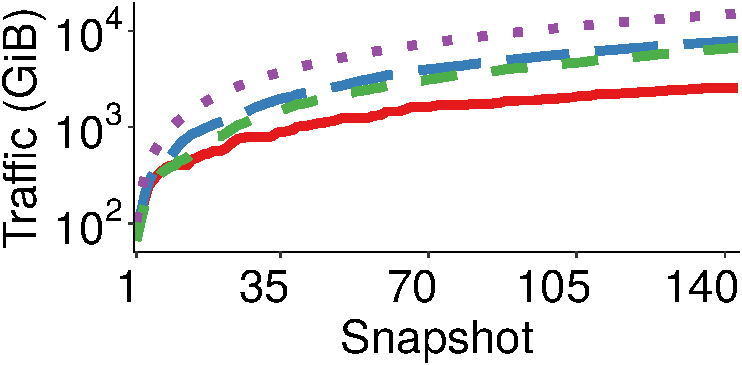
\includegraphics[width=0.47\textwidth]{pic/featurespy/plot/bandwidth/upload_traffic_ms.pdf}                           \\
        {\small (a) FSL}                                                                               & {\small (b) MS}      \\
        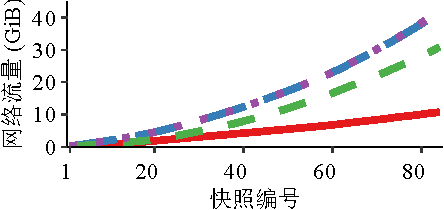
\includegraphics[width=0.47\textwidth]{pic/featurespy/plot/bandwidth/upload_traffic_linux.pdf} &
        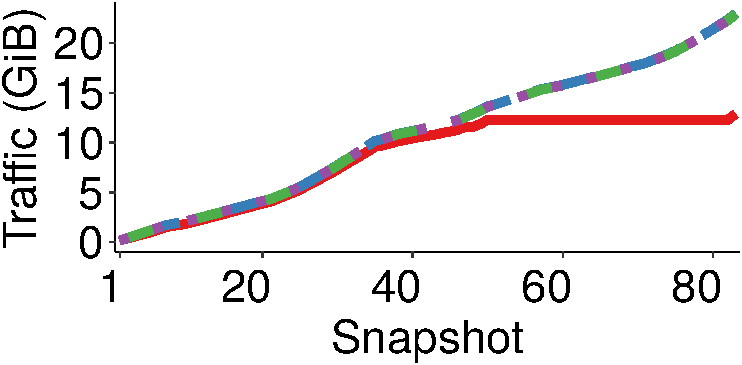
\includegraphics[width=0.47\textwidth]{pic/featurespy/plot/bandwidth/upload_traffic_couch.pdf}                        \\
        {\small (c) Linux}                                                                             & {\small (d) CouchDB}
    \end{tabular}
    \caption{(Exp\#10) 存储每个快照后的累积网络流量。}
    \label{fig:featurespy-expNetworkTraffic}
\end{figure}

图~\ref{fig:featurespy-expNetworkTraffic}展示针对4种数据集的存储流量开销分析结果。由于\prototype 执行纯源端重复数据删除,因此它优于其他所有方法。例如,在存储最后一个快照后,\prototype 将目标端重复数据删除的网络流量在FSL数据集中减少了98.9\%,并在MS数据集中减少了83.1\%。两阶段重复数据删除在FSL数据集中表现良好(例如,相较于\prototype 只有3.7\%的额外带宽开销),这是因为FSL数据集包含大量用户内冗余。但是,在MS数据集中,两阶段重复数据删除的网络流量最终是\prototype 的3.1倍。此外,由于Linux和CouchDB数据集的每个版本内几乎没有冗余,并且需要大量源端重复数据删除查询,对于Linux数据集,它仅带来1.05\%的流量节省,而对于CouchDB数据集,它甚至导致0.31\%额外的流量开销。随机阈值重复数据删除相较于目标端重复数据删除带来的流量节省是完全不同的。在MS数据集中,它带来了55.75\%的流量节省,而在FSL和Linux数据集中,则只有21.60\%和26.68\%。对于CouchDB数据集,其甚至引入了0.0016\%的额外流量开销。另外,本文发现在CouchDB的前35个版本中,几个方案的网络流量几乎是一致的,而对于后面的版本,\prototype 的累计网络流量几乎保持不变。这是因为这35个版本是通用版本(几乎没有冗余),但这些通用版本和社区/企业版本之间存在大量冗余,使得\prototype 不再需要上传大量数据。